\chapter{Oblivious Routing in General Embedded Networks}\label{sec:routing}

\section{Background}\label{sec:routing:background}

Routing algorithms are responsible for finding a path from point A to point B in a given network. There are a variety of competing criteria that go into designing a routing algorithm. Should it be simple and compact? Should it be sensitive to current traffic loads? Should it be determined at compile-time or run-time? Should the path be determined in advance or a node at a time? These questions and more have led to a plethora of routing algorithms designed for all sorts of networks. This chapter will consider the basic types of routing and then present a relatively new method of routing that has never (to the author's knowledge) been implemented in a working system before.

\subsection{Types of Routing Algorithms}\label{sec:routing:background:comparison_routing_algorithms}

Routing algorithms can be divided and sub-divided into a number of groups. The basic organization ad hierarchy of unicast routing algorithms is shown in Figure \ref{fig:routing:taxonomy}.

\begin{landscape}
	\begin{figure}[p]
		\begin{centering}
			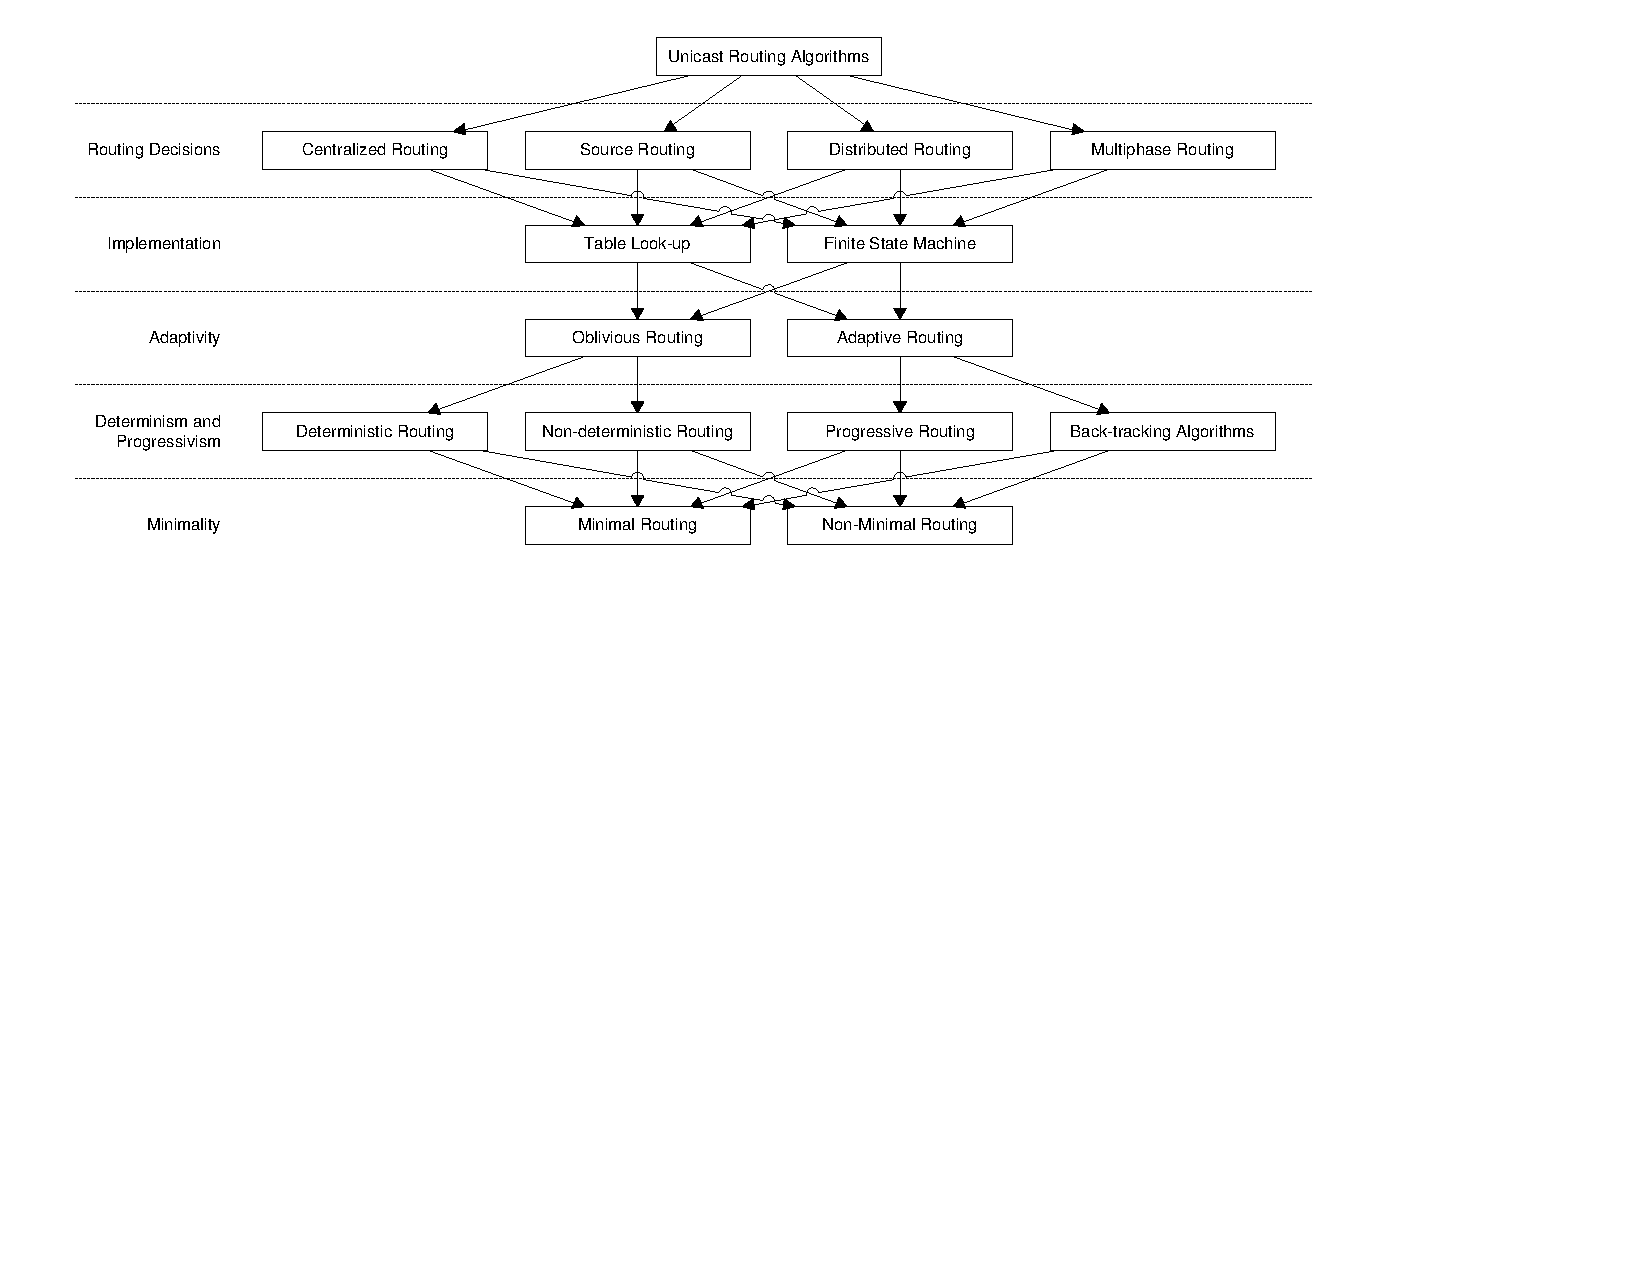
\includegraphics{Routing/Figures/routing-taxonomy.pdf}
			\caption[Taxonomy of Routing Algorithms]{Taxonomy of Routing Algorithms \cite{ref:1997-duato-interconnection_networks}}
			\label{fig:routing:taxonomy}
		\end{centering}
	\end{figure}
\end{landscape}

Routing decisions can generally be classified as centralized, source, distributed, or multiphase. In centralized routing, all routing decisions are made by a centralized controller. In source routing, the routing decisions are completely made by the source of the transmission. In distributed routing, each node in the path decides the next node to take. Combinations of the above can be used, and are called multi-phase routing decisions. For example, the source node could determine a few ``waypoints'' but leave the path from waypoint to waypoint up to the nodes in the path. \cite{ref:1997-duato-interconnection_networks}

Routing algorithms are usually implemented in one of two methods: with a routing table or with a finite state machine. Routing table implementations use a table that is generated either at compile-time or at run-time, and each entry in the table contains information on how to route to a given node. Finite state machines generate a path using a pre-determined state machine to generate a path for each request. \cite{ref:1997-duato-interconnection_networks}

Routing algorithms are generally classified as either oblivious or adaptive. An oblivious routing scheme does not look at the state of the network (e.g. traffic load) when making a routing decision, although it can consider link cost. An adaptive routing algorithm does take the state of the network into consideration when making routing decisions. Adaptive algorithms generally use this information to attempt to lower the congestion in overworked nodes. Adaptive algorithms are more complex than oblivious algorithms, but are historically better at lowering congestion. \cite{ref:1997-duato-interconnection_networks}

Oblivious routing algorithms can be deterministic or non-deterministic. Deterministic routing algorithms, such as Dijkstra's algorithm, always provide the same shortest path between nodes. Non-deterministic oblivious routing algorithms can supply multiple, non-minimal paths, and select between them using randomization techniques. As a result, traffic is spread around the network, thus reducing localized congestion. \cite{ref:2003-racke-oblivious_routing} Adaptive algorithms can be progressive, or can utilize backtracking. A progressive algorithm always sends the packet towards the destination, whereas backtracking allows a packet to travel backwards (usually to attempt a new path). \cite{ref:1997-duato-interconnection_networks}

Routing algorithms can be either minimal or non-minimal. A minimal routing algorithm always supplies the shortest path, or potentially paths if there is more than one path of the same shortest length. A non-minimal path can supply paths that are not the shortest. One implication is that minimal algorithms always send a packet closer to the destination, and thus backtracking algorithms cannot be minimal. \cite{ref:1997-duato-interconnection_networks}

\subsection{Oblivious Routing in General Networks}\label{sec:routing:background:oblivious_routing}

While it may seem that adaptive routing is clearly superior to oblivious routing, in reality adaptive routing is more complex than oblivious routing. Adaptive routing also requires nodes to send data to each other so that nodes know what traffic is like at other nodes, which increases overall traffic. Researchers have recently begun focusing on oblivious routing for special applications where the overhead and complexity of adaptive routing are undesirable.  Oblivious routing has been under study for a long time, but oblivious routing had only been applied to specific types of networks and was not suitable for arbitrary networks until relatively recently. In 2002, a mechanism was finally devised that allowed oblivious routing to be applied to any arbitrary network. The rest of this section is devoted to explaining that mechanism as described by Harald R\"a cke in \cite{ref:2003-racke-oblivious_routing}. R\"acke's method is a source routing, table-lookup based non-minimal, non-deterministic oblivious routing scheme.

\subsubsection[Preliminaries]{Preliminaries}\cite{ref:2003-racke-oblivious_routing} \label{sec:routing:background:oblivious_routing:preliminaries}

The network is modeled as an undirected graph $G$ with nodes $V$  and edges $E=V\times V $. The number of nodes is $n=|V| $ and the weight of an edge (i.e. link capacity) is $b:V\times V \rightarrow \mathbb{R}^+_0 $. It is assumed that the weights are normalized such that the minimum connected weight is 1 and the maximum weight is $b_{\textrm{max}} $. Note that if $b(u,v)=0 $  then the nodes $U$ and $V$ are not connected. The function $\textrm{cap}:2^V \times 2^V \rightarrow \mathbb{R}^+_0 $  represents the aggregate capacity between the two sets of nodes $X,Y \subseteq V $ and is defined as:

\[
\textrm{cap}(X,Y):=\sum_{x\in X,y\in Y} b(x,y)
\]
	
The capacity leaving a set $X \subseteq V $  is defined as $\textrm{out}(X)=cap(X,\overline{X}) $, where $\overline{X}:=V\setminus X $.

\subsubsection[The Bisimulation Technique]{The Bisimulation Technique \cite{ref:2003-racke-oblivious_routing}}\label{sec:routing:background:oblivious_routing:bisimulation_technique}

R\"acke's method works by transforming general networks into a tree network, finding the desired path, and then transforming the path back to the general network. This process is called the bisimulation technique. Trees are used because finding paths in tree networks is trivial.
 
The first step in the routing algorithm is to transform a given problem instance $I$ (i.e. a routing request between nodes $u,v\in V $) on $G$ to a problem instance $I_t$ on $T$. $I$ is translated onto $T$ using a previously determined mapping $\pi _1:V\rightarrow V_t $. When a message is sent between two nodes $u,v\in V $, as defined in $I$, a corresponding message is sent between two nodes $\pi _1(u),\pi _1(v)\in V_t $. 

The second step involves finding the path between nodes $\pi _1(u),\pi _1(v)$, which is the solution to $I_t$. To find a path in a tree network, one simply needs to find the two paths to the root node from nodes $\pi _1(u),\pi _1(v)$, concatenating the two paths at the root, and then removing any common intermediate nodes.

The third step is to transform the solution to $I_t$ back onto $G$. This is done using the randomized mapping $\pi _2:V_t\rightarrow V $, where $\pi _2(\pi _1(v))=v, \forall v\in V $. This mapping is randomized (i.e. selects one of many paths at random) because there are typically more nodes in $T$ than in $G$, which means that one node in $G$ is represented by multiple nodes in $T$ and thus there are multiple paths in $G$ given a single path in $T$.

\subsubsection[The Virtual Tree Network]{The Virtual Tree Network \cite{ref:2003-racke-oblivious_routing}}\label{sec:routing:background:oblivious_routing:virtual_tree_network}

The virtual tree network is constructed using a hierarchical decomposition $\mathscr{H} $. $\mathscr{H} $ starts with graph $G$ and partitions it into smaller sub-graphs. These sub-graphs are recursively partitioned until the last sub-graphs contain a single node in $G$. A graph is partitioned such that the cut is of minimum sparsity\footnote{The concept of a sparsest cut for a graph in this context is based on linear Programming and concurrent multicommodity flows, which are far too complex for this discussion. For information on this topic, see \cite{ref:2003-racke-oblivious_routing} and \cite{ref:1993-ahuja-network_flows}.}, which minimizes congestion in the network. This decomposition process describes a natural tree, where a node's children are the sub-graphs partitioned from that node's graph. The tree that results, $T_\mathscr{H} $, is called the decomposition tree corresponding to $\mathscr{H} $, and each node corresponds to a set $H=\{ v: v \in V\} $ in $G$. An example decomposition is shown in Figure \ref{fig:routing:ex_hierarchical_decomposition}.

\begin{landscape}
	\begin{figure}[p]
		\begin{centering}
			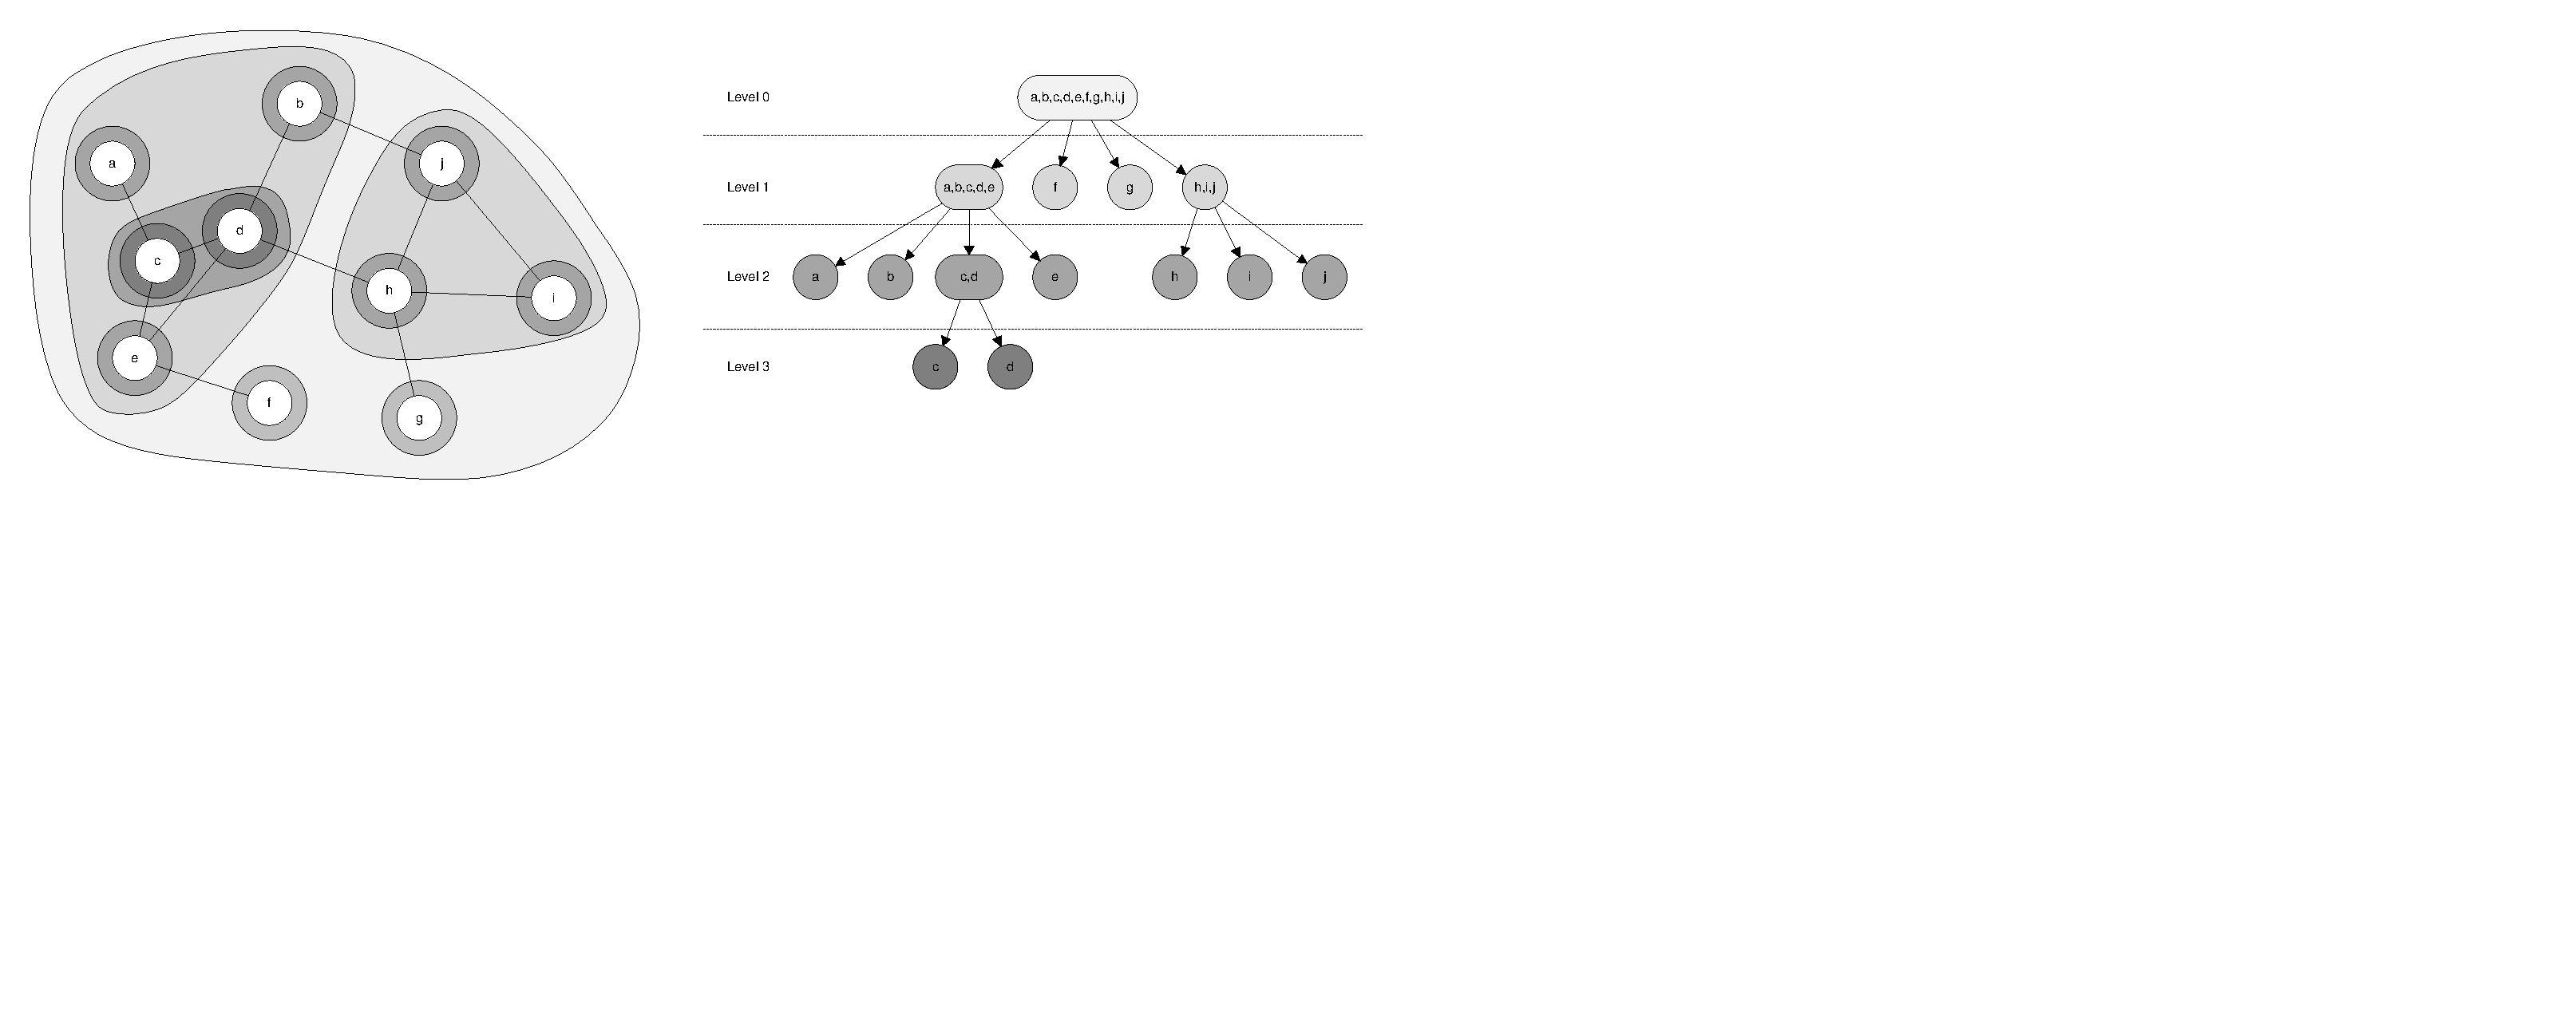
\includegraphics[width=8.5in]{Routing/Figures/routing-ex_hierarchical_decomposition.pdf}
			\caption{Example Hierarchical Decomposition}
			\label{fig:routing:ex_hierarchical_decomposition}
		\end{centering}
	\end{figure}
\end{landscape}

The tree has several properties that are needed for later. The bandwidth of an edge in the tree is defined as $b_t(u_t,v_t):=\textrm{cap}(U,V) $. The level of a node in the tree is defined as the number of nodes between it and the root node. The weight of a level is defined by the function $w_l:2^V\rightarrow \mathbb{R}^+_0 $  for every level $l\in \{ 0,...,\textrm{height}(T_\mathscr{H} )\} $ and is defined as:

\[
w_l(X):=\sum_{\begin{array}{c} 
e\in X\times V \\ 
level(e)\leq l \\
\end{array}} \textrm{cap}(e)
\]

Informally, the weight is the capacity of all edges leaving the set for nodes in the higher level nodes. A Concurrent Multi-Commodity Flow (CMCF) problem, from linear programming theory is defined for each cluster in the hierarchical decomposition. The CMCF for node $H_v $ has a commodity $d_{u,v} $ for each ordered pair $u,v\in H_v $. The source for the commodity is $u$, the sink is $v$, and the demand is defined as:

\[
\textrm{dem}(u,v):=\frac{w_{l+1}(u)\cdot w_{l+1}(v)}{w_{l+1}(H_v)}
\]

The flow for the commodity along an edge in $T_\mathscr{H} $  is decomposed\footnote{The idea of flow decomposition is a linear programming technique that is outside the scope of this paper. See \cite{ref:1993-ahuja-network_flows} for more information.} into a set of convex paths between the endpoints. A path is selected from the set based on a randomized weighting according to $\frac{\textrm{weight}(p)}{\textrm{weight}(P)} $ for a path $p\in P $ from the convex set.

\section{Objectives}\label{sec:routing:objectives}

The routing algorithm must meet the following criteria: 
\begin{enumerate}
	\item Self-configuring
	\item Applicable to general networks
	\item Utilize communication resources efficiently
	\item Utilize processing resources appropriately
\end{enumerate}
As with the network, data link, and physical layers, the routing algorithm must be completely self-configuring to make it easy to use. In addition, the routing algorithm must be applicable to any type of network in order to avoid constraining the application developer. The routing algorithm must be appropriate to both the communication and processing resources available. In other words, it should avoid congestion and shouldn't need to communicate much to support routing. Quick computation of routing tables and path selections must be possible. Of course these last few points are contradictory, so a balance needs to be struck.

\section{Methodology}\label{sec:routing:methodology}

R\"acke's method will be used for this project because it has the advantage of being applicable to general networks, which satisfies the second objective, and not needing the state of the network, which helps satisfy the third objective. The primary downside to R\"acke's method is that solving CMCF's involves using techniques from linear programming that are NP-complete (i.e. unsolvable by computers). Approximations do exist, such as the ellipsoidal method proposed by R\"acke himself, but even these methods are still too complex to implement effectively on embedded hardware. To make R\"acke's method suitable for embedded systems, the sparsest cut calculation and path decomposition must be replaced with elements that are simple to compute. This will, unfortunately, nullify some of the bounds on congestion that were determined for the method, but that is deemed as necessary. The routing algorithm is divided into two sections: routing tree generation and path selection.

\subsection{Routing Tree Generation}\label{sec:routing:methodology:routing_tree_generation}

The steps for generating the routing tree are:
\begin{itemize}
	\item Generate graph $G=(V,E) $ from the node information
	\item Decompose the graph into tree network $T_\mathscr{H} $
	\item Calculate the tree node weights $w_l(X), \forall X\in T_\mathscr{H} $
\end{itemize}
Graph $G=(V,E) $ is generated using the neighbor information obtained via the report neighbors protocol command. The list of nodes and edges are stored in a single data structure called an adjacency matrix $M$. If two nodes $u,v\in V $ are connected, then $M(u,v)=M(v,u)=1 $, otherwise $M(u,v)=M(v,u)=0 $. By this definition, $M$ is symmetrical along the diagonal. $M(u,u) $ is technically undefined, although is set to 0 in practice.

To decompose the graph, a graph partitioning algorithm must first be devised. A partitioning algorithm that performs a single cut (i.e. divides the graph in two) is simpler to implement than an algorithm that could potentially perform multiple cuts, so a binary partitioning algorithm is used. The minimal paths between all of the nodes in the (sub)graph are calculated first. The longest minimal path, $\mathscr{P} $, is found, the length, $l_\textrm{path} $, is calculated, and the endpoints of the path, $u_\textrm{end},v_\textrm{end}\in \mathscr{P} $. The nodes are then sorted according to their distance from $u_\textrm{end} $, and a cut-point, $c$, is set for the middle of the sorted list. All nodes that are below the cut-point are grouped with $u_\textrm{end} $, and the rest of the nodes are grouped with $v_\textrm{end} $. In some cases this method can lead to nodes being grouped together that are far apart geographically if the network is not well distributed. In this case, a rule of thirds is applied: if the distance between $c$ and $u_\textrm{end} $, $c_\textrm{dist} $, is less than $l_\textrm{path}/3 $ or greater than $2\cdot l_\textrm{path}/3 $, then $c$ is shifted until $l_\textrm{path}/3 \leq c_\textrm{dist} \leq 2\cdot l_\textrm{path}/3 $. An example is shown in Figure \ref{fig:routing:example_graph_partition}. This process is repeated until the leaves of the tree only contain graphs with a single node. An example decomposition is shown in Figure \ref{fig:routing:example_binary_decomposition}.

\begin{figure}[ptb]
	\begin{centering}
		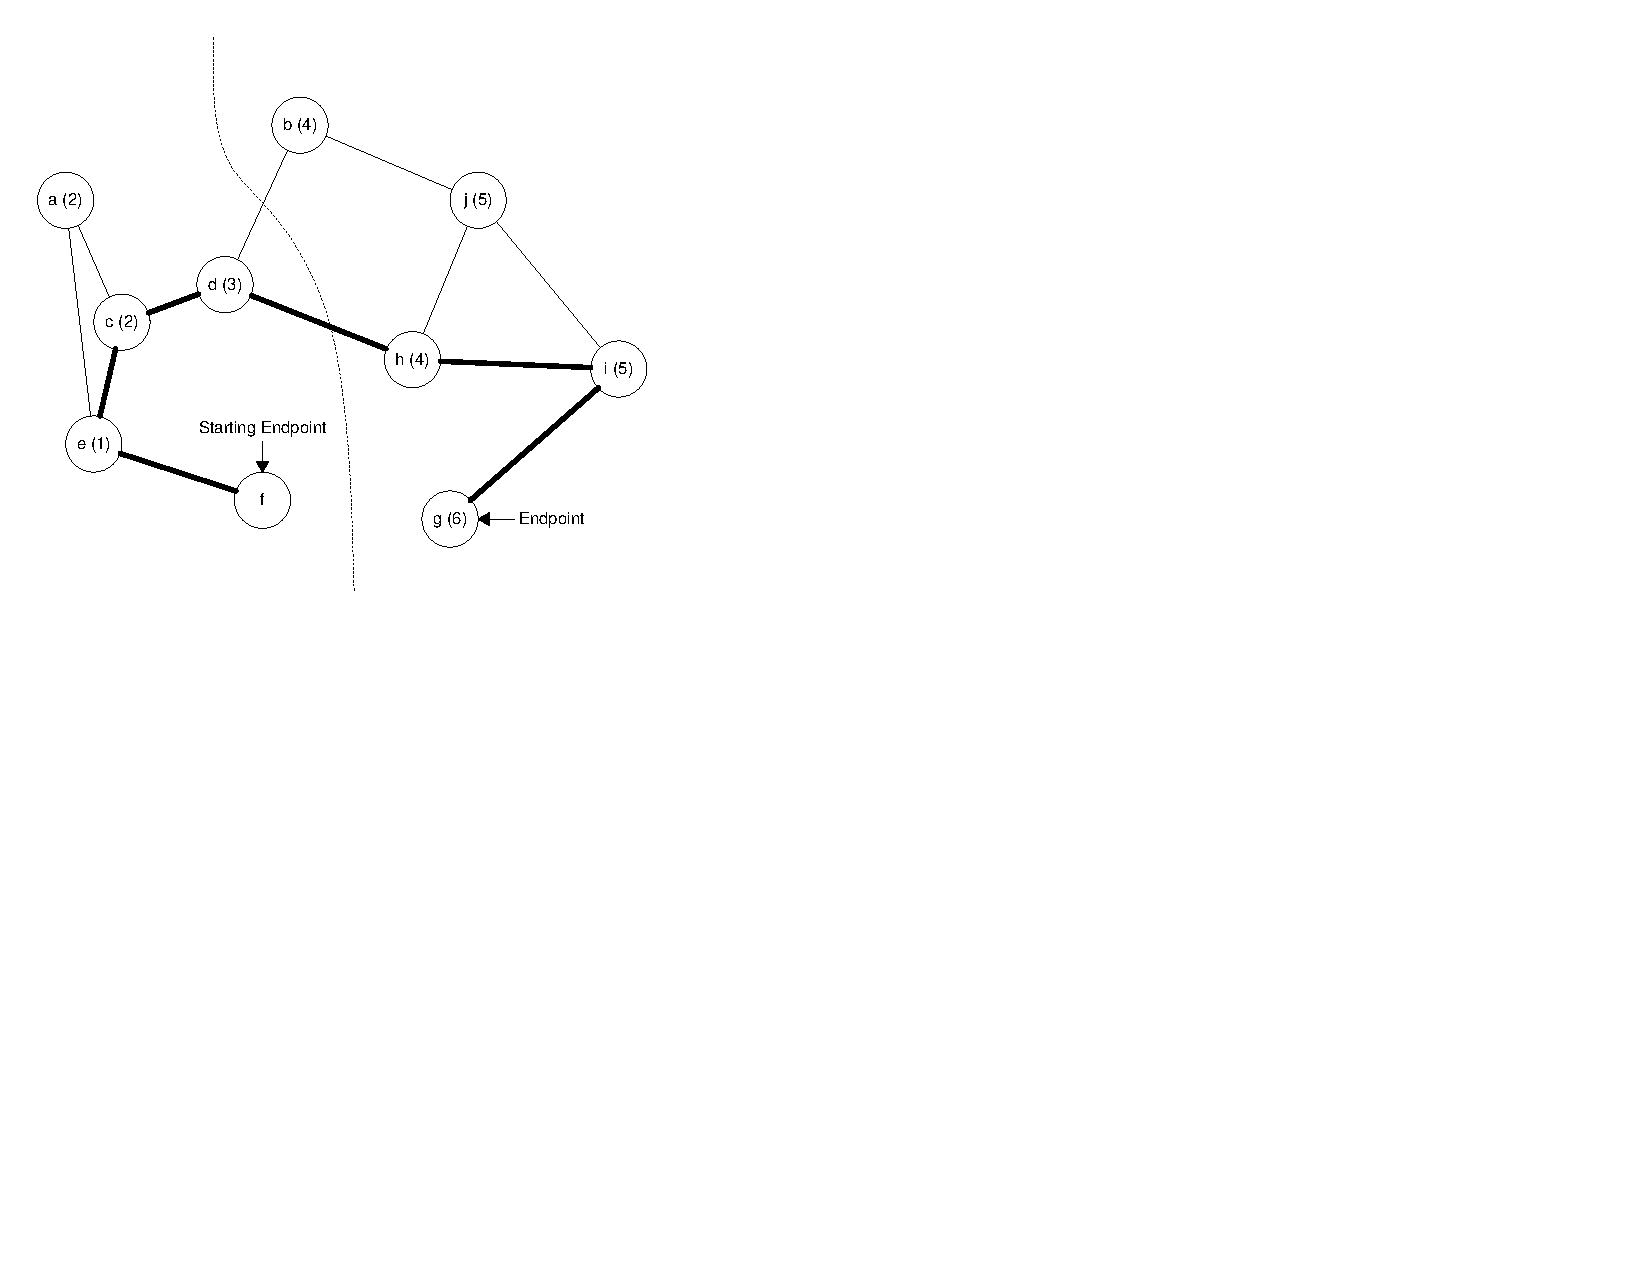
\includegraphics{Routing/Figures/routing-example_graph_partition.pdf}
		\caption{Example graph partition}
		\label{fig:routing:example_graph_partition}
	\end{centering}
\end{figure}

\begin{landscape}
	\begin{figure}[p]
		\begin{centering}
			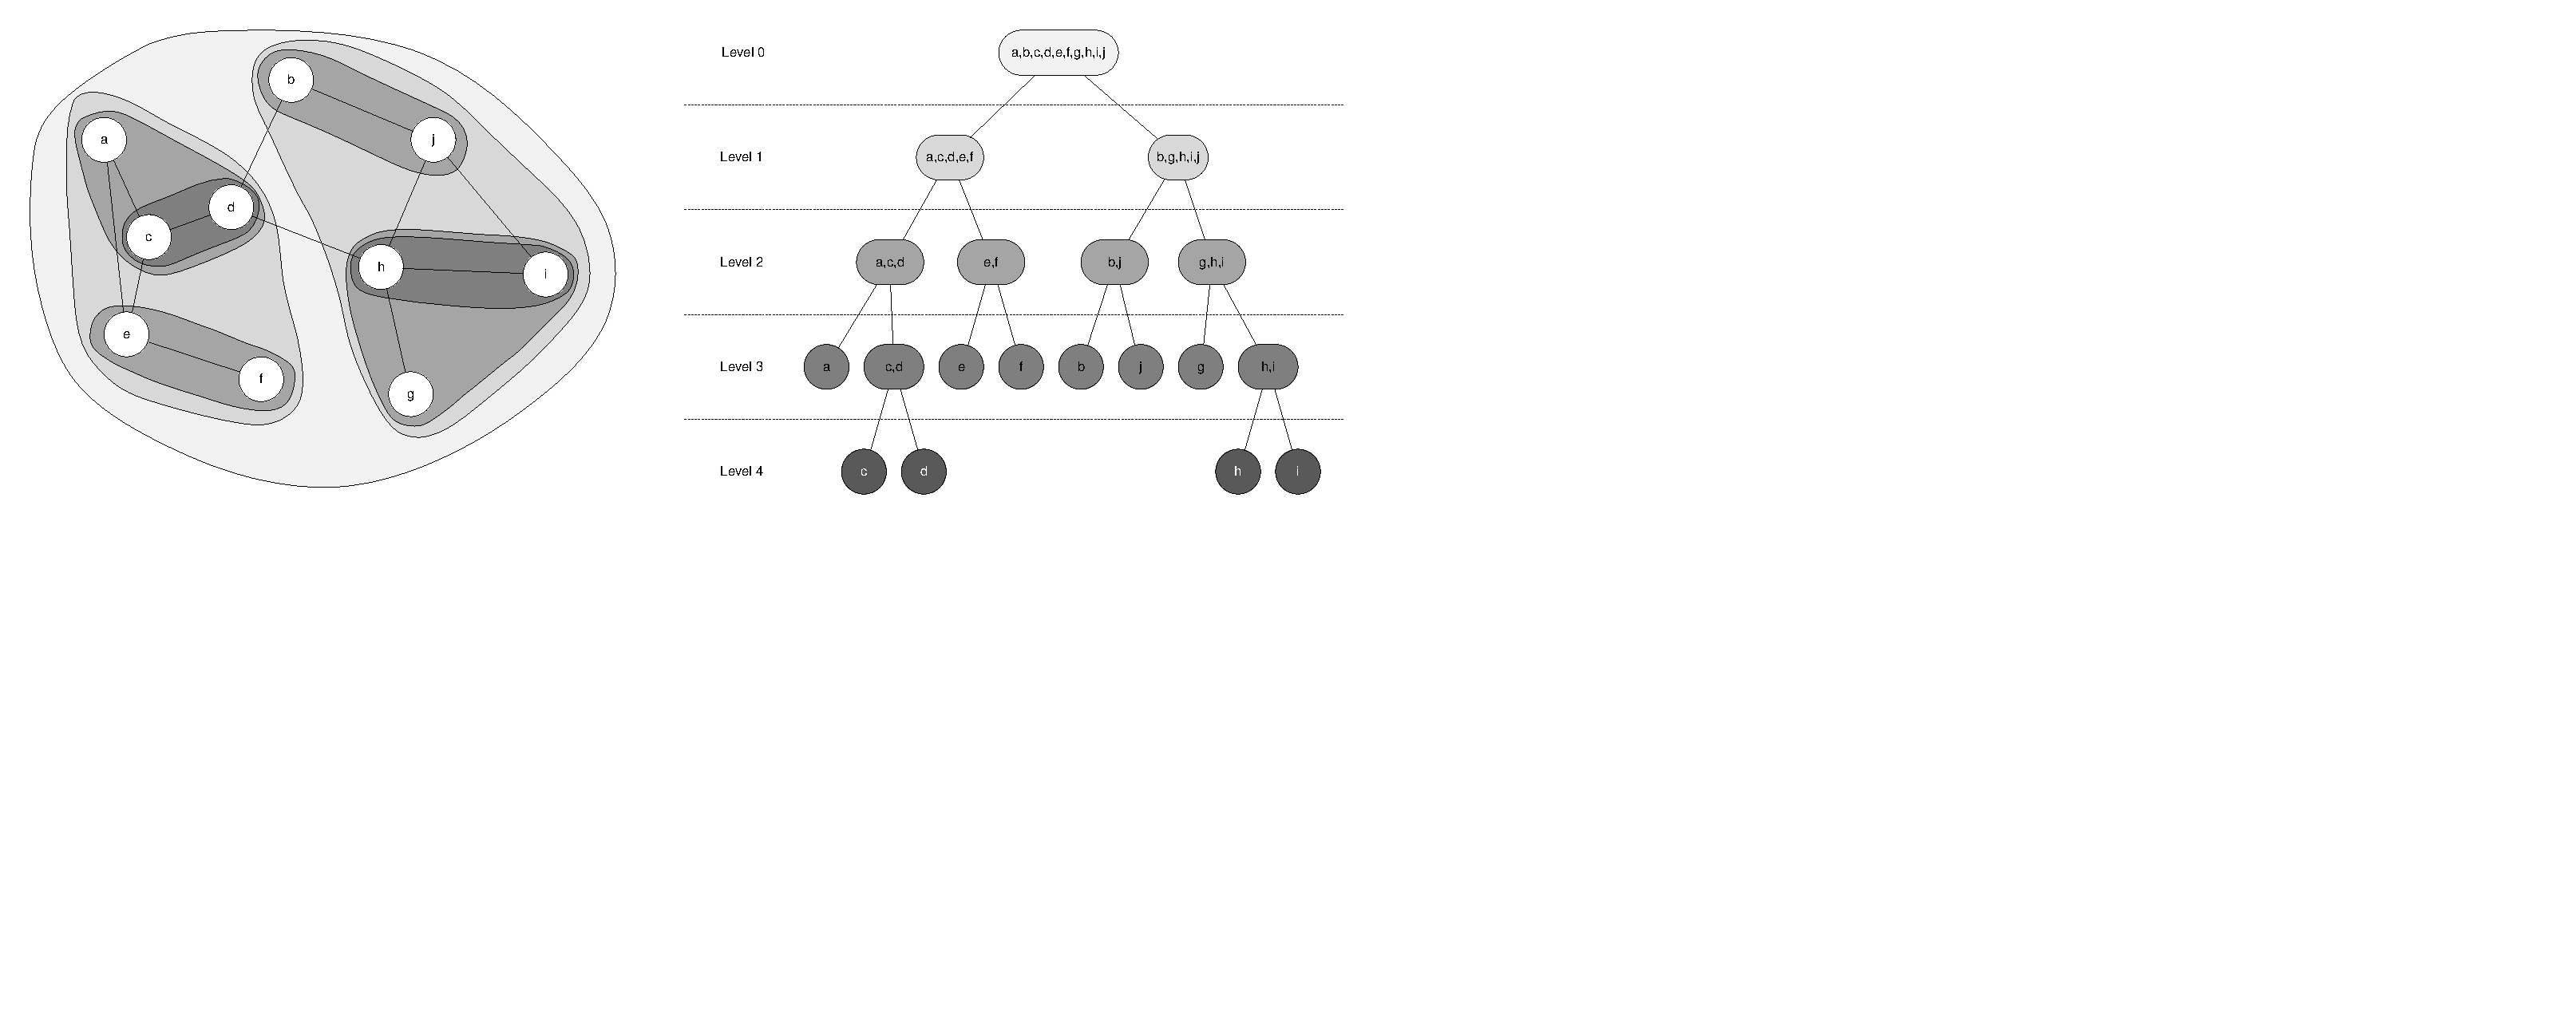
\includegraphics[width=8.5in]{Routing/Figures/routing-example_binary_decomposition.pdf}
			\caption{Example Binary Decomposition}
			\label{fig:routing:example_binary_decomposition}
		\end{centering}
	\end{figure}
\end{landscape}

The weights for each node are calculated using the formula from Section \ref{sec:routing:background:oblivious_routing} for node capacity:
\[
w_l(u\in X):=\frac{\textrm{cap}(u)}{\textrm{cap}(X)}
\]

This formula states that the weight is defined as the normalized bandwidth between node $u$ and all graph nodes in the tree node's parent. For the root node, the capacity is defined as the total capacity of the network.

After the tree is generated, it can be distributed to the rest of the system via the new routing table available and request routing table commands. The tree isn't a routing table in the strictest sense, but it serves the same purpose as a routing table.

\subsection{Path Selection}\label{sec:routing:methodology:path_selection}

The first step in determining the path that a packet will take is to find the path in the tree network, $\mathscr{P}_T $. This is done by find the path from the source leaf to the tree root, the path from the destination leaf to the tree root and concatenating the paths. An example is shown in Figure \ref{fig:routing:example_tree_path}.

\begin{landscape}
	\begin{figure}[ptb]
		\begin{centering}
			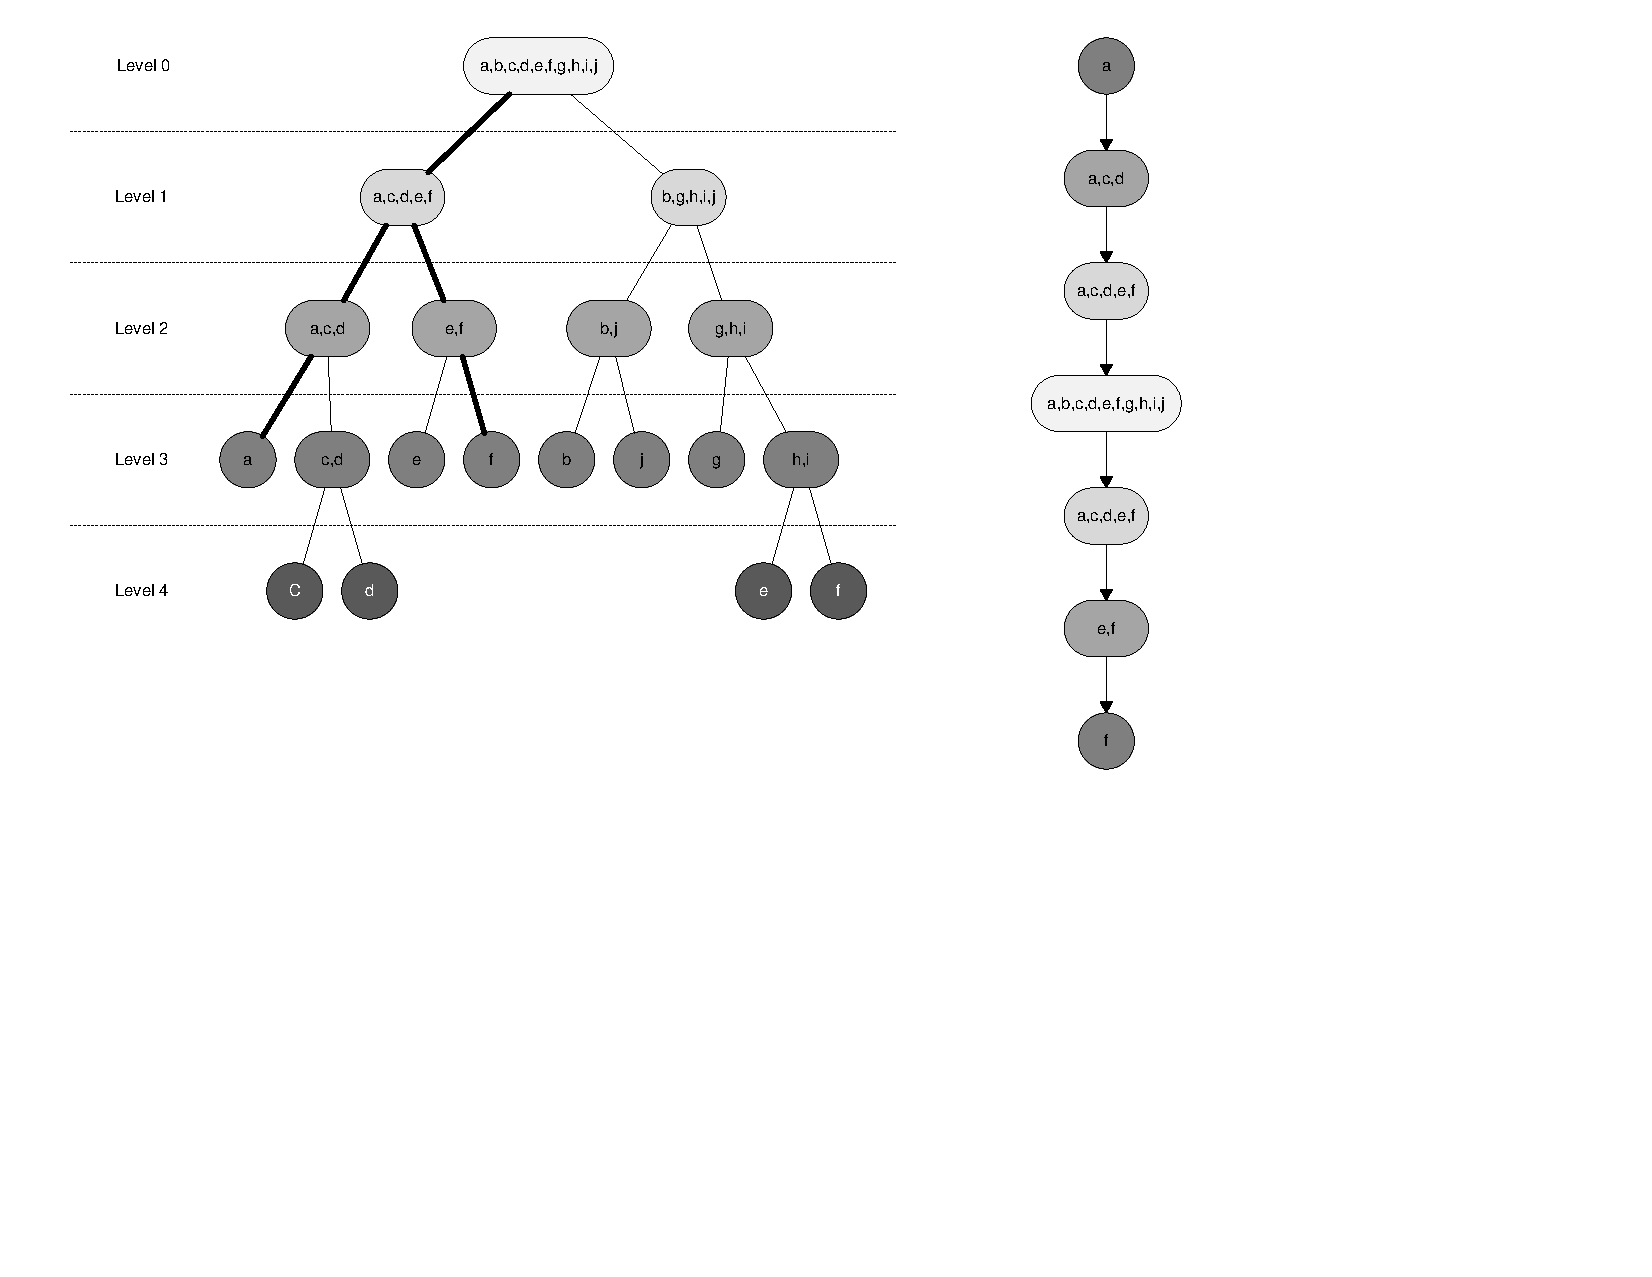
\includegraphics[width=8.5in]{Routing/Figures/routing-example_tree_path.pdf}
			\caption{Example Tree Path}
			\label{fig:routing:example_tree_path}
		\end{centering}
	\end{figure}
\end{landscape}

The next step is to select a path $\mathscr{P} $  comprised of nodes in $G$ from $\mathscr{P}_T $. This is done by generating randomized values for each node in a subgraph, and selecting based on this randomization and the weight. A side effect of not using linear programming to solve this problem is that sometimes a selected path gets ``stuck,'' where there are no nodes in the next subgraph connected to the currently selected subgraph. In this case, the algorithm backtracks to the previous tree node, marks the previously selected graph node as invalid, and tries again. An example path selection is shown in Figure \ref{fig:routing:example_path_selection}.

\begin{figure}[ptb]
	\begin{centering}
		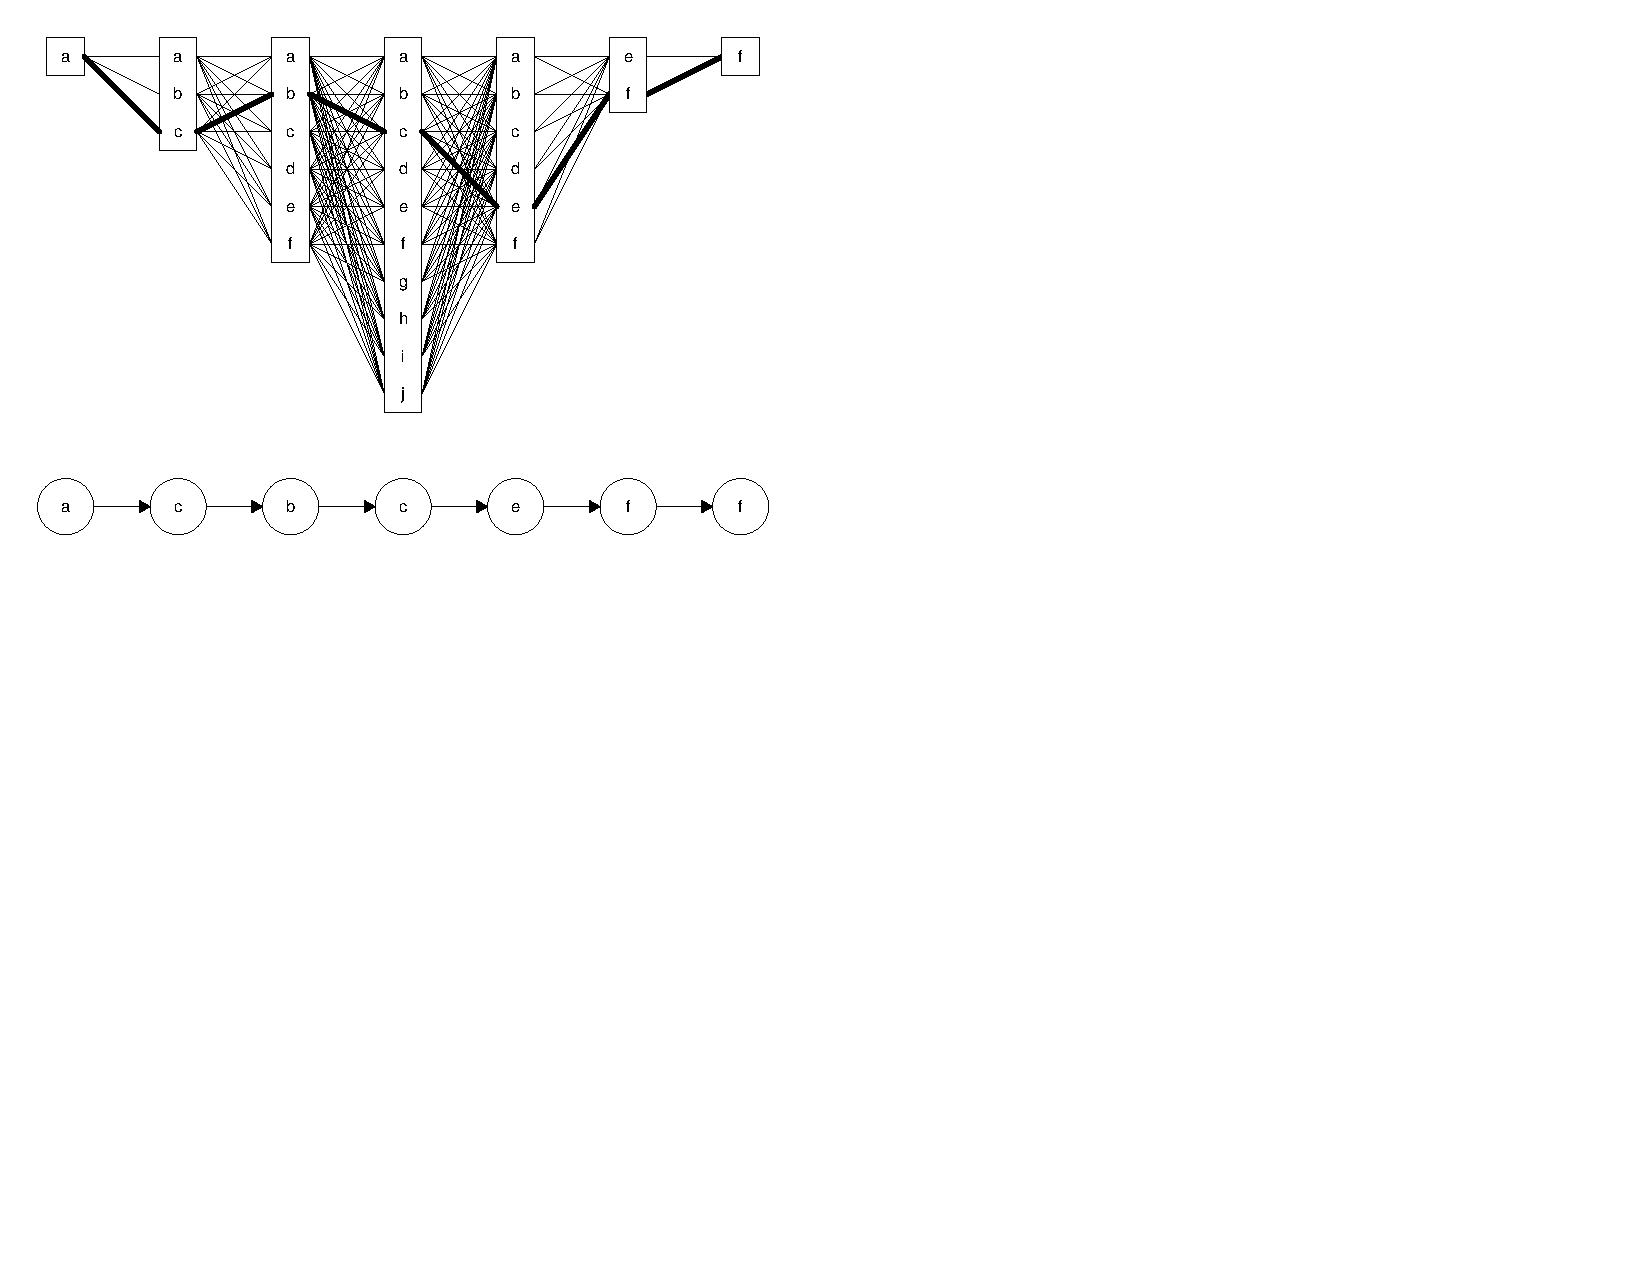
\includegraphics{Routing/Figures/routing-example_path_selection.pdf}
		\caption{Example path selection}
		\label{fig:routing:example_path_selection}
	\end{centering}
\end{figure}

The final step is to remove any redundant graph nodes. Nodes may be repeated in direct succession, or there may be other nodes in between, in which case this represents a path cycle. Once this is complete a valid path has been selected. An example path reduction is shown in Figure \ref{fig:routing:example_path_reduction}.

\begin{figure}[ptb]
	\begin{centering}
		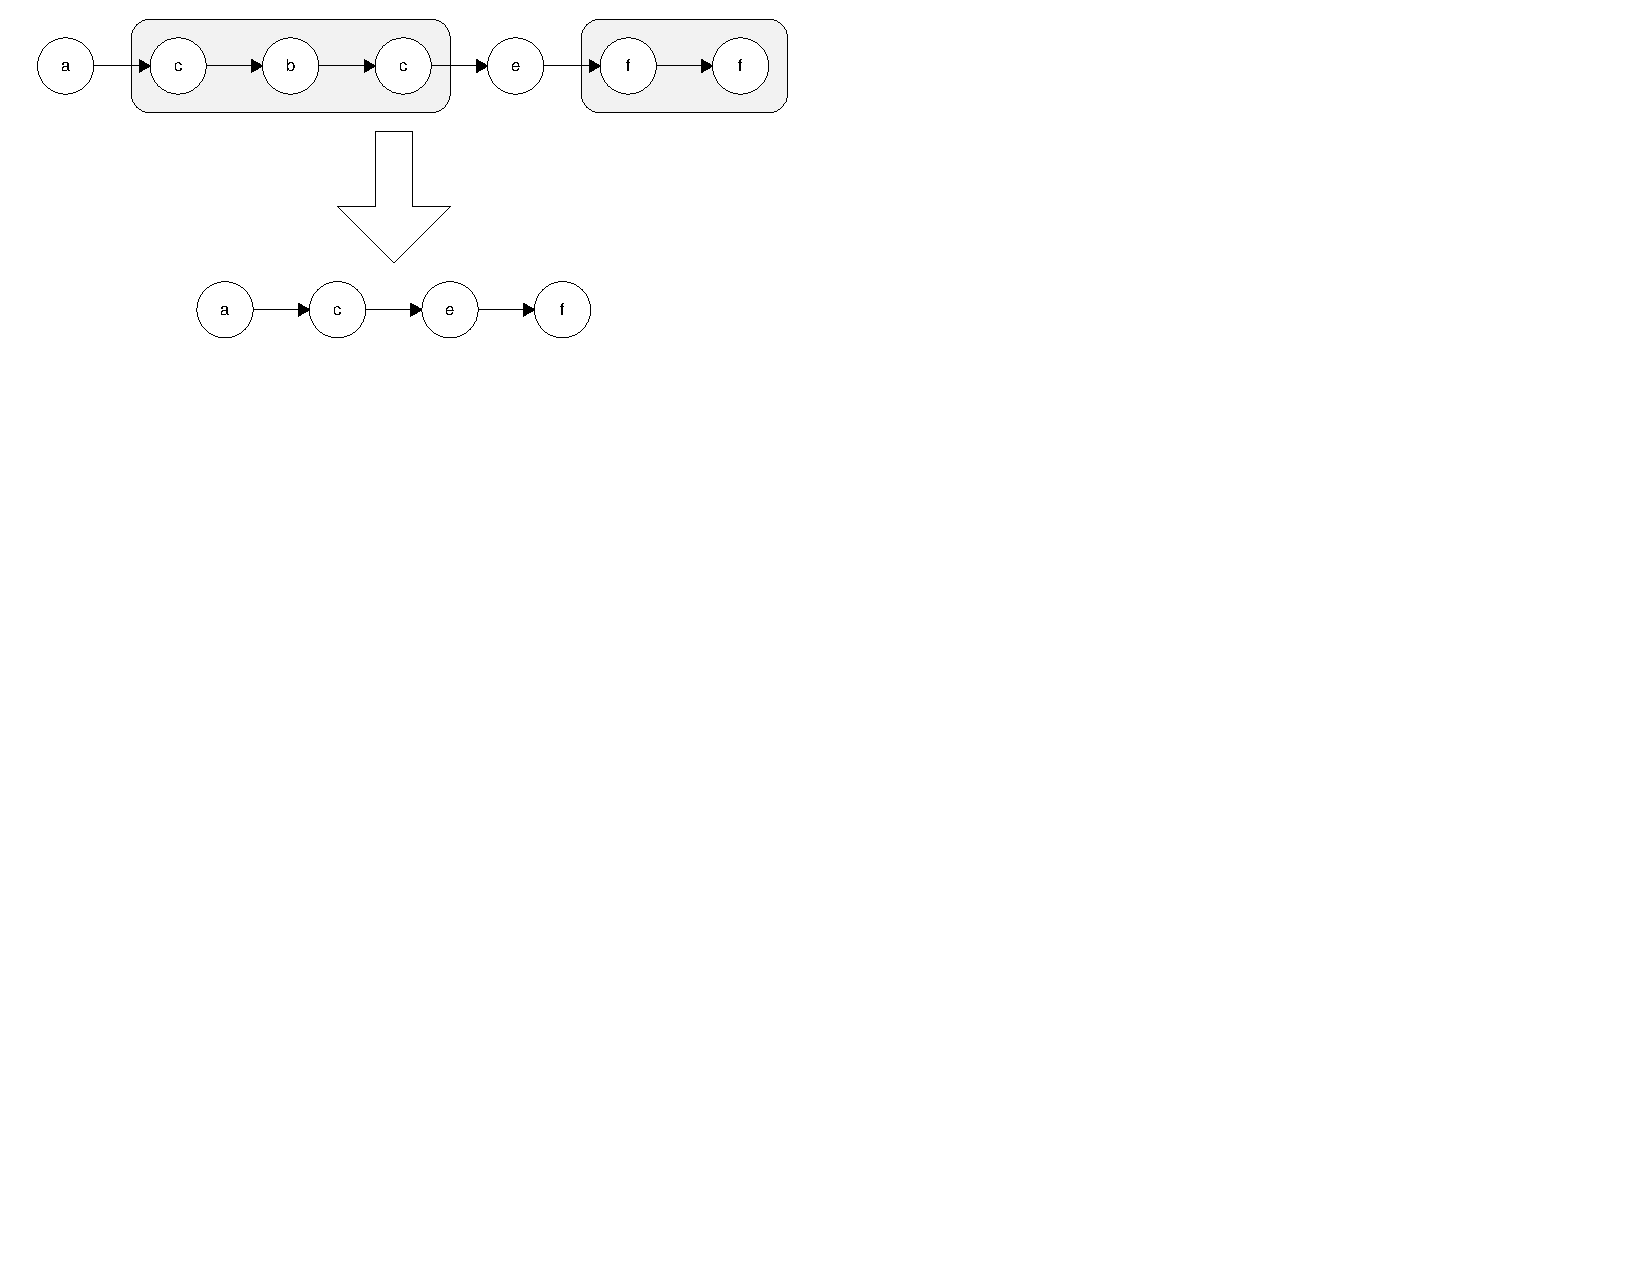
\includegraphics{Routing/Figures/routing-example_path_reduction.pdf}
		\caption{Example reduced path}
		\label{fig:routing:example_path_reduction}
	\end{centering}
\end{figure}

\section{Implementation}\label{sec:routing:implementation}

\subsection{Routing Tree Generation}\label{sec:routing:implementation:routing_tree_generation}

The first step in the routing algorithm is, once again, generating the graph. In practice, an edge list is created before the adjacency matrix to aid in speeding up later steps. Edges are represented by a tuple consisting of the addresses of the two endpoint nodes. Each tuple is always ordered with the lower address first, and the list of tuples is ordered first by the lower address, then by the upper address. When an edge is added to the edge list, it is also added to the adjacency matrix. An adjacency matrix is used because determining whether or not two nodes are connected only requires a single lookup operation and no loops, which greatly increases performance. This is important because the routing algorithm checks this information many times, thus even slight increases in performance here result in large performance increases aggregately.

The second step in the routing algorithm is to generate the tree decomposition. The set of all minimal paths is created before the partitioning process begins to save computation time during the partitioning process. The algorithm for creating the minimal path list is borrowed from \cite{ref:2007-lau-java_library_of_graph_algorithms}, and is essentially a modified version of Dijkstra's algorithm that re-uses information between destinations. The algorithm is shown in Algorithm \ref{alg:routing:shortest_minimal_paths}.
\begin{algorithm}
	\caption[Shortest Minimal Path]{Shortest Minimal Path Algorithm \cite{ref:2007-lau-java_library_of_graph_algorithms}}
	\begin{algorithmic}[1]
		\STATE \textbf{given} $n$ nodes and $m$ edges
		\STATE \textbf{find} the shortest paths, $S(i)$, given $i=2,...,n $ from node 1 to all others
		\STATE \textbf{set} $p=1, k=n, S(1)=0$
		\REPEAT
		\FOR{$i=1,2,...,n $}
			\STATE \textbf{set} $L(i)=i, S(i)=\infty $
		\ENDFOR
		\FORALL{$i=2,3,...,n$}
			\STATE \textbf{let} $j=L(i)$
			\STATE $S(j)=\textrm{min}\left( S(j),S(p)+1\right) $
			\IF{$S(j)$ is less than the current minimum}
				\STATE \textbf{set} $q=j, t=i$
			\ENDIF
		\ENDFOR
		\STATE \textbf{set} $p=q, L(t)=L(k),k=k-1$
		\UNTIL{$k=1$}
	\end{algorithmic}
	\label{alg:routing:shortest_minimal_paths}
\end{algorithm}

To partition a (sub)graph, the algorithm first checks if there are two nodes because that is a special case. If there are two nodes, then the two nodes are split and the branch is finished. If there are more than two nodes, then the longest path is found by comparing the minimal paths between all nodes in the (sub)graph. After the path is found, the distance from the start endpoint to all of the other nodes is found, and all of the nodes are sorted according to distance. The cut-point is calculated and the rule of thirds is checked. If the rule of thirds fails, then the cut-point is shifted until the rule is satisfied. After the groups have been determined, the new child nodes of a parent node are created. If there are two or more nodes in the new child node, then the partition algorithm is called again. The complete partition algorithm is shown in Algorithm \ref{alg:routing:partition_algorithm}.
\begin{algorithm}
	\caption{Partition Algorithm}
	\begin{algorithmic}[1]
		\STATE \textbf{given} minimal path set $\mathscr{P}_{\textrm{min}} $  and (sub)graph $G_p$
		\IF{$|\mathscr{P}|=2 $}
			\STATE split $G_p$ into two child nodes $G_{c_1}$ and $G_{c_2}$, each containing one graph node
		\ELSE
			\STATE find $p_{\textrm{max}}\in \mathscr{P}_{\textrm{min}_p} $, where $\mathscr{P}_{\textrm{min}_p}\in \mathscr{P}_\textrm{min} $ is the minimal path set for $G_p$
			\STATE sort the nodes in $G_p$ according to distance from an endpoint $u_\textrm{end}\in p_{\textrm{max}} $
			\STATE \textbf{set} $c=\left| G_p\right| $
			\IF{$c_\textrm{dist} \le l_\textrm{path}/3 $ \OR $c_\textrm{dist} \ge 2\cdot l_\textrm{path}/3 $}
				\STATE Shift $c$ until $l_\textrm{path}/3 \leq c_\textrm{dist} \leq 2\cdot l_\textrm{path}/3 $
			\ENDIF
			\STATE group nodes below $c$ with $u_\textrm{end} $ and nodes above $c$ with $v_\textrm{end} $
			\STATE create child nodes of $G_p$, $G_{c_1}$ and $G_{c_2}$, containing the two groups
			\IF {$\left| G_{c_1}\right| \ge 1 $ \OR $\left| G_{c_2}\right| \ge 1 $}
       \STATE partition child nodes
			\ENDIF
		\ENDIF
	\end{algorithmic}
	\label{alg:routing:partition_algorithm}
\end{algorithm}

Node weights are pretty simple to calculate. The capacity between a graph node in a child tree node $G_c$ and all graph nodes in $G_p$ is calculated and stored as the weight directly. The values are not normalized here because the process would require the path selection to use floating point math, which is slow on devices that don't have a hardware floating point unit, such as the F2808. The algorithm is shown in Algorithm \ref{alg:routing:weight_algorithm}.

\begin{algorithm}
	\caption{Node Weight Algorithm}
	\begin{algorithmic}[1]
		\STATE \textbf{given} (sub)graph $G_c$ and it's tree node parent $G_p$
		\FORALL{$v\in G_c$}
			\STATE \textbf{set} $w_l(v)=\textrm{cap}(v,G_p) $
		\ENDFOR
	\end{algorithmic}
	\label{alg:routing:weight_algorithm}
\end{algorithm}

\subsection{Path Selection}\label{sec:routing:implementation:path_selection}

The tree path between the source and destination is found by first creating a path from the source to the root, and the destination to the root. This is done by starting at the source/destination and storing the parent as the next step in the path. The parent of the parent is then stored, and so on to the root. Redundant nodes between the source and destination paths are then removed here, instead of later on, to gain efficiency. Starting with the source node, probabilities are generated by multiplying the weights and a random number for each graph node. The node with the highest probability is selected, and the process repeats itself at the next tree node. Before the probabilities are calculated, each node is checked for connectivity with the previously selected node, and if not the probability is set to 0. If all probabilities in a given tree node are set to 0, then the algorithm backtracks to the previous tree node, marks the previously selected node as a dead end by marking its probability as 0, and tries again. When the full path is selected, redundant nodes are removed to form a simple path. The full algorithm is shown in Algorithm \ref{alg:routing:path_selection}.

\begin{algorithm}
	\caption{Path Selection Algorithm}
	\begin{algorithmic}[1]
		\STATE \textbf{given} source node $u$ and destination node $v$
		\STATE remove redundant parts of $\mathscr{P}_{t_u} $ and $\mathscr{P}_{t_v} $ (i.e. path subsets $\mathscr{P}_{t_{u_s}}=\mathscr{P}_{t_{v_s}} $)
		\STATE concatenate $\mathscr{P}_{t_u} $ and $\mathscr{P}_{t_v} $ to form $\mathscr{P}_t $
		\STATE \textbf{set} the current tree node index, $x$, to point to the source node $u$ (i.e. to index 1)
		\REPEAT
			\STATE generate random numbers, $R$, for all nodes in the next tree node
			\STATE \textbf{set} $P=R\cdot W $ for all node weights $W$
			\STATE store graph node, $g$, with the highest probability $p\in P>0 $  to the network path $\mathscr{P} $
			\IF{ there is no $p>0 $}
				\STATE decrement $x$
				\STATE mark the previous node $g$ with $p=0$
			\ELSE
				\STATE increment $x$
			\ENDIF
		\UNTIL{$x$ points to $v$}
		\STATE remove any redundant nodes in $\mathscr{P} $
	\end{algorithmic}
	\label{alg:routing:path_selection}
\end{algorithm}

\section{Results}\label{sec:routing:results}

The routing algorithm is checked for correctness by viewing the results of the routing tree generation for two networks: one regular and well distributed, the other somewhat irregular. The regular network and its resulting decomposition tree are shown in Figure \ref{fig:routing:test_1}. The algorithm gives a very nice decomposition tree that is a well-balanced, full tree. The first cut divided the network in half along its shorter axis, which encourages transmissions among nodes on one side of the network to stay in that network.

\begin{landscape}
	\begin{figure}[ptb]
		\begin{centering}
			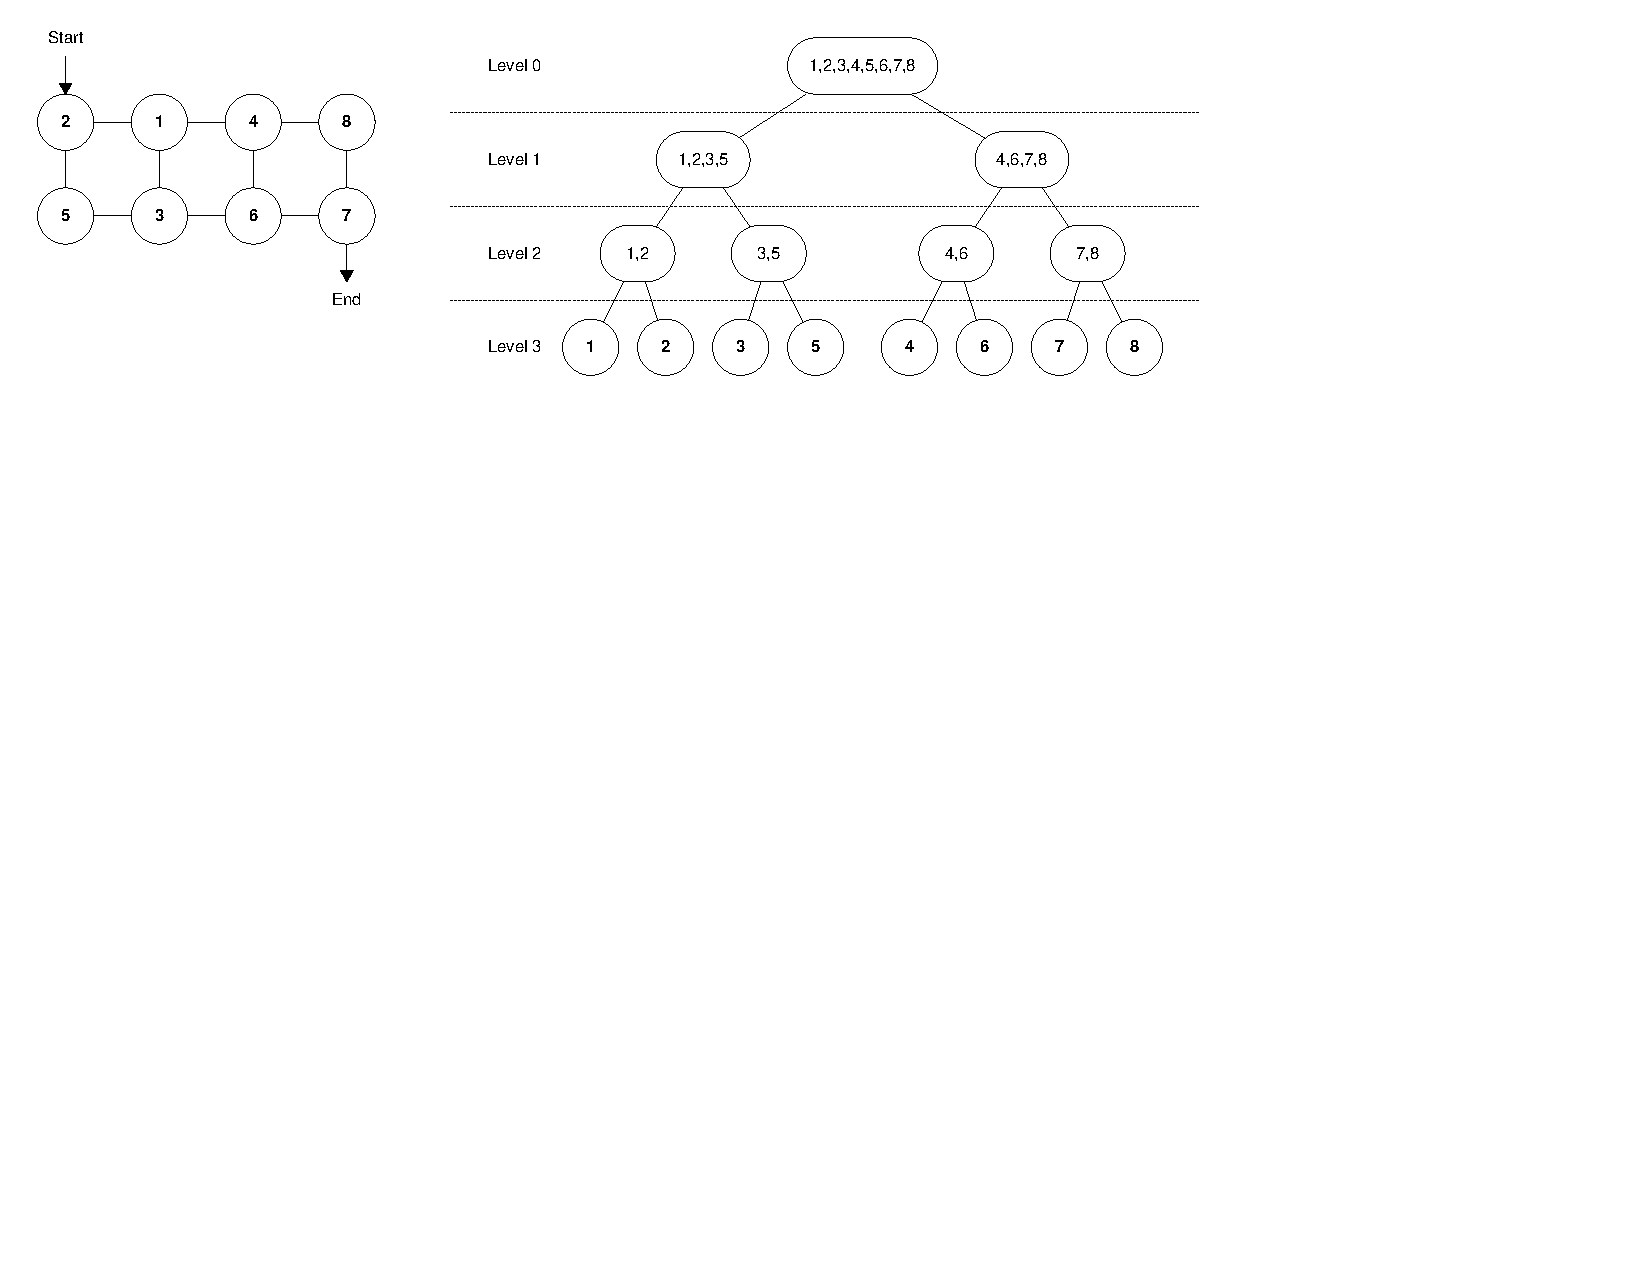
\includegraphics[width=8.5in]{Routing/Figures/routing-test_1.pdf}
			\caption{Test network 1 and the resulting decomposition tree}
			\label{fig:routing:test_1}
		\end{centering}
	\end{figure}
\end{landscape}

The second network is much more irregular in design, and so produces a more irregular tree, with the results in Figure \ref{fig:routing:test_2}. The tree still divided the network pretty well, although it couldn't quite figure out what to do with node 7. The network consists of two somewhat distinct parts, with node 7 straddling the middle, which is why node 7 is spun off so quickly, which is actually not a bad decision because it means each side of the network will have equal access, in terms of path lengths, to this node. The decision to lump nodes 2 and 4 together instead of nodes 2 and 8 may not be quite ideal, but it's not bad either.

\begin{landscape}
	\begin{figure}[ptb]
		\begin{centering}
			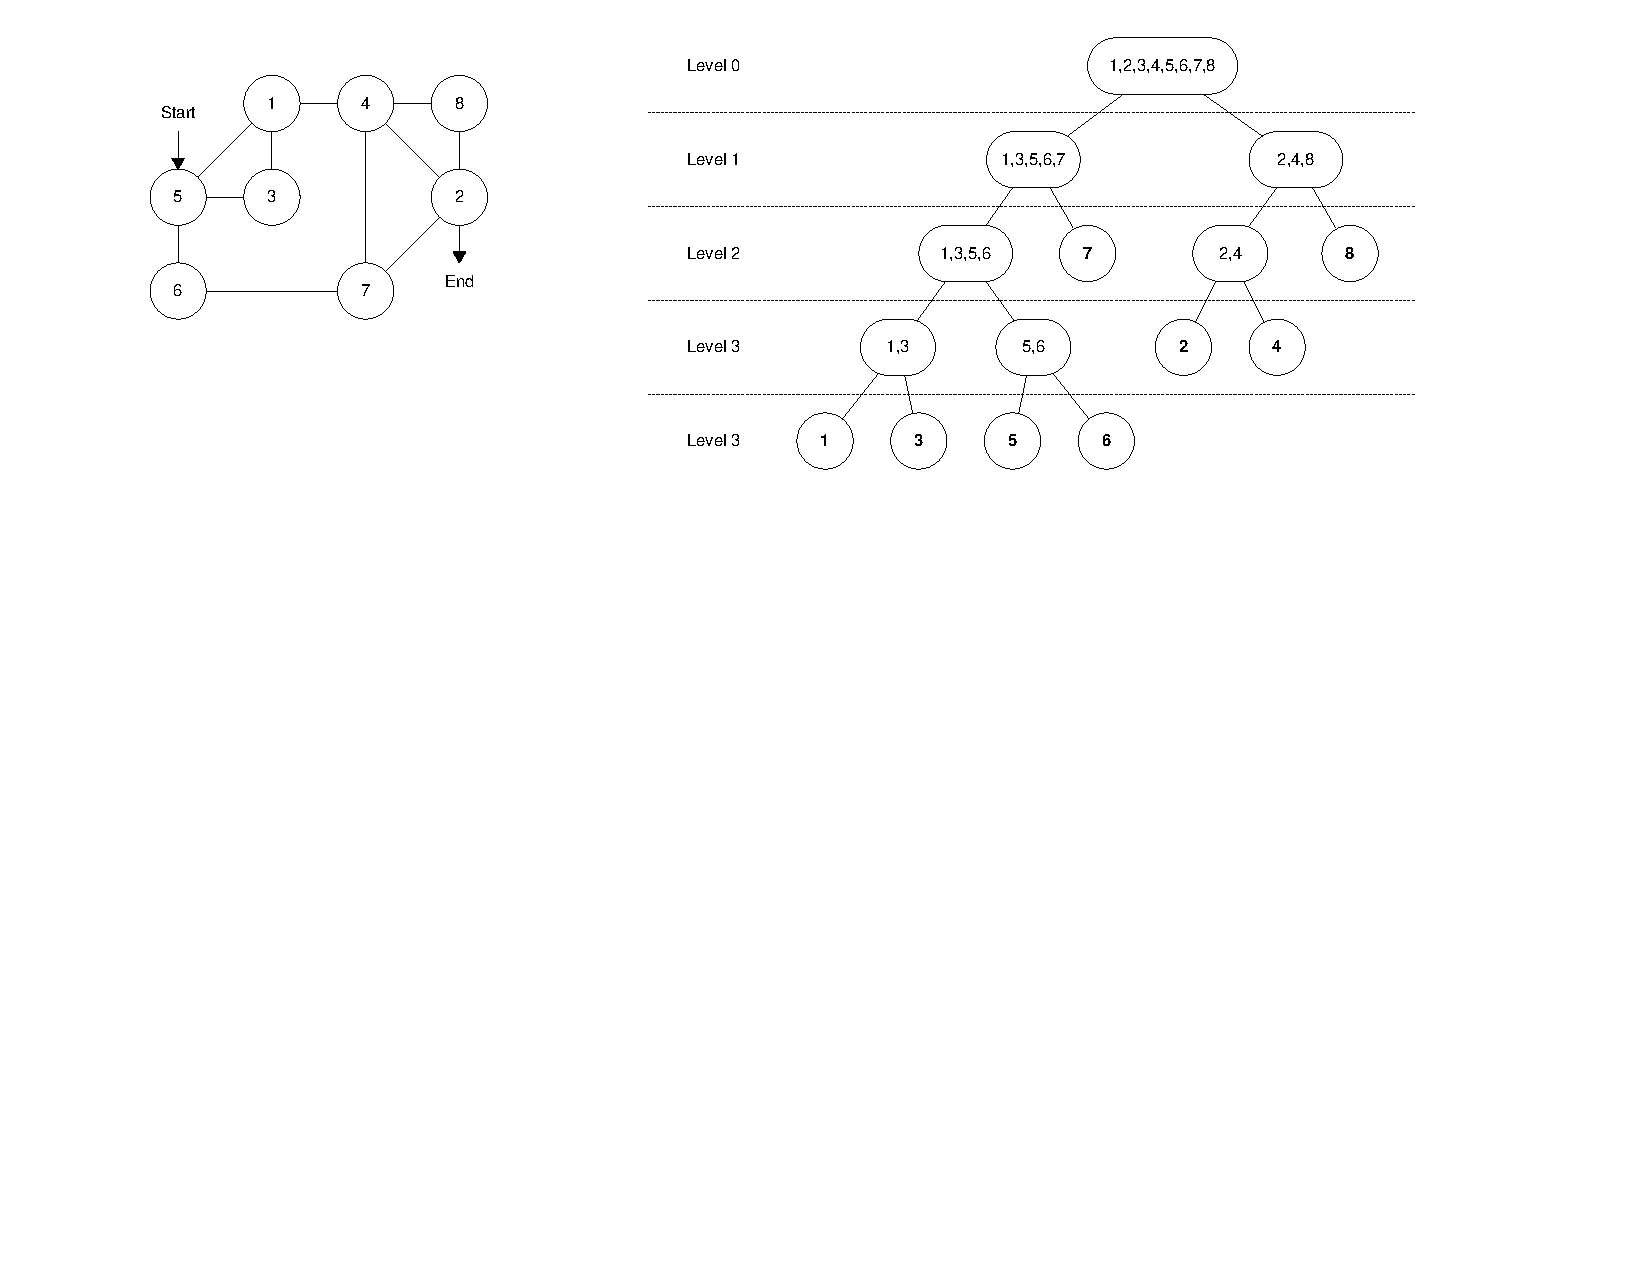
\includegraphics[width=8.5in]{Routing/Figures/routing-test_2.pdf}
			\caption{Test network 2 and the resulting decomposition tree}
			\label{fig:routing:test_2}
		\end{centering}
	\end{figure}
\end{landscape}

The next test is to determine the frequency that alternate paths are taken. The network from test 1 is used for the first test and paths from node 2 to node 7 are calculated. The results are in Table \ref{tab:routing:test_1_paths}. Four paths exist that are the shortest possible between nodes 2 and 7, and the routing algorithm selected all four of them. It also selected a more out of the way path on one occasion. This is the type of behavior that is desired because it favors the best path, but still distributes the traffic across the network. 

\begin{table}
	\begin{center}
		\setlength{\extrarowheight}{1.5pt}
		\caption{Test 1 path selection results}
		\vspace{0.1cm}
		\begin{tabular} {|l|c|}
			\hline
			\textbf{Path} & \textbf{Times selected (out of 100)} \\
			\hline
			\hline
			$2\Rightarrow 1\Rightarrow 4\Rightarrow 8\Rightarrow 7 $ & 62 \\
			\hline
			$2\Rightarrow 1\Rightarrow 4\Rightarrow 6\Rightarrow 7 $ & 10 \\
			\hline
			$2\Rightarrow 1\Rightarrow 3\Rightarrow 6\Rightarrow 7 $ & 20 \\
			\hline
			$2\Rightarrow 5\Rightarrow 3\Rightarrow 6\Rightarrow 7 $ & 7 \\
			\hline
			$2\Rightarrow 1\Rightarrow 3\Rightarrow 6\Rightarrow 4\Rightarrow 8\Rightarrow 7 $ & 1 \\
			\hline
		\end{tabular}
		\label{tab:routing:test_1_paths}
	\end{center}
\end{table}

The network from test 2 is used for the second test and paths from node 5 to node 2 are calculated. The results are in table \ref{tab:routing:test_2_paths}. This test showed a good distribution, once again. There are two shortest paths available, and the algorithm took both of them. It did also take a slightly longer path some of the time, but definitely favored one of the shortest paths most of the time.

\begin{table}
	\begin{center}
		\setlength{\extrarowheight}{1.5pt}
		\caption{Test 2 path selection results}
		\vspace{0.1cm}
		\begin{tabular} {|l|c|}
			\hline
			\textbf{Path} & \textbf{Times selected (out of 100)} \\
			\hline
			\hline
			$5\Rightarrow 1\Rightarrow 4\Rightarrow 2 $  & 77 \\
			\hline
			$5\Rightarrow 3\Rightarrow 1\Rightarrow 4\Rightarrow 2 $  & 11 \\
			\hline
			$5\Rightarrow 6\Rightarrow 7\Rightarrow 2 $  & 12 \\
			\hline
		\end{tabular}
		\label{tab:routing:test_2_paths}
	\end{center}
\end{table}

\section{Future Work}\label{sec:routing:future_work}

Some rather obvious improvements exist that can be made. One of the reasons that R\"acke's work was so important is that it proved oblivious routing is competitive with adaptive routing in regard to traffic. By modifying the algorithm, those bounds no longer apply. In the future, the bounds that do apply to this system could be found. A more intelligent partitioning algorithm could be conceived as well that would surely improve the bounds. Methods such as k-means clustering are worth investigating.

\section{Conclusions}\label{sec:routing:conclusions}

In this chapter, a routing mechanism has been presented that is based on Harald R\"acke's oblivious routing method. The mechanism works by mapping a general network onto a tree network. A path in the network is determined by finding the related path in the tree network and mapping it back to the general network. When the tree network is mapped back to the general network, multiple paths exist within the mapping that can be taken. Weights are assigned to the general graph nodes in the tree network based on their level of connectivity to the nodes in the tree nodes parent. Variable paths that tend toward the shorter paths are selected by mixing these weights with a random number generator. The mechanism produces routing trees that are sensible and well balanced. The mechanism works well and usually, but not always, selects the shortest available path(s) while also spreading the traffic around the network to reduce congestion. 


